%%%%%%%%%%%%%%%%%%%%%%%%%%%%%%%%%%%%%%%%%%%%%%%%%%%%%%%%%%%%%%%%%%%%%%
%
% Institut für Rechnergestuetzte Automation
% Forschungsgruppe Industrial Software
% Arbeitsgruppe ESSE
% http://security.inso.tuwien.ac.at/
% lva.security@inso.tuwien.ac.at
%
% Version 2014-04-10
% 
%%%%%%%%%%%%%%%%%%%%%%%%%%%%%%%%%%%%%%%%%%%%%%%%%%%%%%%%%%%%%%%%%%%%%%

\documentclass[12pt,a4paper,titlepage,oneside]{scrartcl}
\usepackage{esseProtocol}

%%%%%%%%%%%%%%%%%%%%%%%%%%%%%%%%%%%%%%%%%%%%%%%%%%%%%%%%%%%%%%%%%%%%%%
%
% FOR STUDENTS
%
%%%%%%%%%%%%%%%%%%%%%%%%%%%%%%%%%%%%%%%%%%%%%%%%%%%%%%%%%%%%%%%%%%%%%%

% Group number or "0" for Lab0
\newcommand{\gruppe}{2}
% Date
\newcommand{\datum}{2014-05-16}
% valid values: "Lab0", "Lab1" (be sure to use Uppercase for first character)
\newcommand{\lab}{Lab1}

% name of course
\newcommand{\lvaname}{IT Security in Large IT Infrastructures}
% number of course
\newcommand{\lvanr}{183.633}
% year and term, for example: "SS 2012", "WS 2012", "SS 2013", etc.
\newcommand{\semester}{SS 2014}

% Student data in Lab0 or 1. student of group in Lab1
\newcommand{\studentAName}{Ren\'{e} Czerny}
\renewcommand{\studentAMatrnr}{0825750}
\newcommand{\studentAEmail}{e0825750@student.tuwien.ac.at}

% 2. student of group in Lab1, for Lab0 or if your group has less students, remove these 3 lines
\newcommand{\studentBName}{Andreas Riegler}
\renewcommand{\studentBMatrnr}{1028878}
\newcommand{\studentBEmail}{e1028878@student.tuwien.ac.at}

% 3. student of group in Lab1, for Lab0 or if your group has less students, remove these 3 lines
\newcommand{\studentCName}{Klaus Walla}
\renewcommand{\studentCMatrnr}{1028877}
\newcommand{\studentCEmail}{e1028877@student.tuwien.ac.at}

%%%%%%%%%%%%%%%%%%%%%%%%%%%%%%%%%%%%%%%%%%%%%%%%%%%%%%%%%%%%%%%%%%%%%%
%
% DO NOT CHANGE THE FOLLOWING PART
%
%%%%%%%%%%%%%%%%%%%%%%%%%%%%%%%%%%%%%%%%%%%%%%%%%%%%%%%%%%%%%%%%%%%%%%

\newcommand{\lang}{de}
\newcommand{\colormode}{color}
\newcommand{\dokumenttyp}{Abgabedokument \lab}

\begin{document}

\maketitle
\setcounter{section}{0}
\setcounter{tocdepth}{2}
\tableofcontents

%%%%%%%%%%%%%%%%%%%%%%%%%%%%%%%%%%%%%%%%%%%%%%%%%%%%%%%%%%%%%%%%%%%%%%
%
% CONTENT OF DOCUMENT STARTS HERE
%
%%%%%%%%%%%%%%%%%%%%%%%%%%%%%%%%%%%%%%%%%%%%%%%%%%%%%%%%%%%%%%%%%%%%%%

\section{Lab1a}

\subsection{Report}

\subsection{Example exploit}
ChatterBox in der jetztigen Version ist anf"allig f"ur Session Hijacking. Da die gesamte Daten"ubertragung unverschl"usselt erfolgt kann ein Angreifer z.B. mittels Packet Sniffing Session-IDs stehlen oder auch sogar an Login-Daten gelangen.
\newline
\newline
Beispiel:
\newline
Ein Benutzer loggt sich "uber ein unverschl"usseltes WLAN an einem ChatterBox-Server ein. Ein Angreifer k"onnte nun den Datenverkehr mithilfe eines Packet Sniffers (z.B. Wireshark) mitlesen und so die Session-ID, die bei jedem HTTP-Request/Response mitgeschickt wird, dieses Benutzers erhalten (\hyperref[fig:message]{siehe Abbildung~\ref*{fig:message} auf Seite~\pageref*{fig:message}}).
\begin{figure}[h!]
  \centering
  \fbox{
    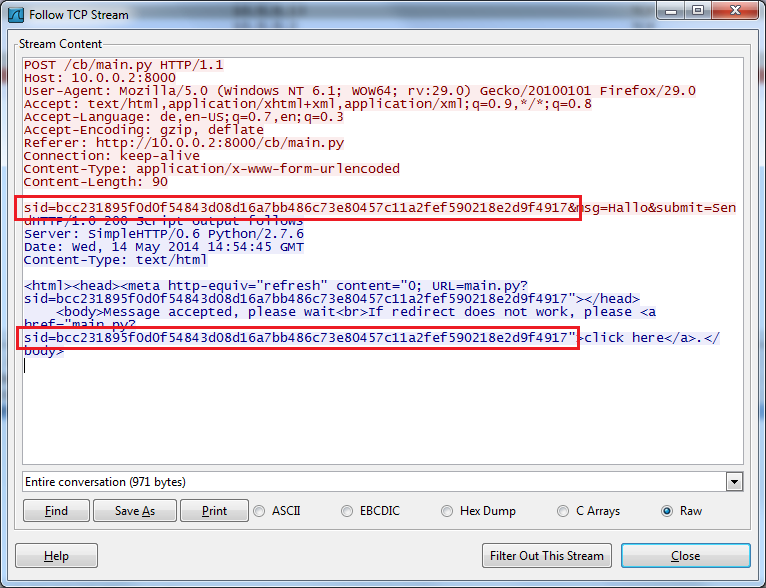
\includegraphics[width=0.8\textwidth]{./imgs/send_message.png}
  }
  \caption{Benutzer schickt eine Message ab}
  \label{fig:message}
\end{figure}
\newline
\newline
Mittels dieser Session-ID erh"alt der Angreifer nun Zugriff auf den Account des Benutzers indem er die gestohlene ID "uber die URL angibt (\lstinline{http://<Server-IP>:8000/cb/main.py?sid=<gestohlene SID des Benutzers>}).

\subsection{Executive summary}
%\emph{Hinweise:}
%\begin{itemize}
%    \item Verwenden Sie entweder diese deutsche Version oder die englische Version der Vorlage in \lstinline{protocol.tex}
%    \item Setzen Sie alle Variablen nach \emph{FOR STUDENTS} im .tex-File
%    \item Ersetzen Sie die Platzhalter für Ihren Namen und Ihre MatNr.
%    \item Löschen Sie diesen Abschnitt über Hinweise und die folgenden Beispiel-Kapitel
%    \item Achten Sie auf geforderte Formate und Anforderungen an die Dateinamen für Ihre lab-Abgabe.
%    \item Führen Sie \lstinline{pdflatex} mindestens 2 Mal aus, damit die Referenzen und Seitenzahlen richtig im PDF dargestellt werden
%    \item Sie können dazu auch das Makefile verwenden: \lstinline{make de}
%\end{itemize}
\section{Lab1b}

\subsection{Sub-Ueberschrift 1}
Lorem ipsum dolor sit amet, consetetur sadipscing elitr, sed diam nonumy eirmod tempor invidunt ut labore et dolore magna aliquyam erat, sed diam voluptua. 

\subsection{Sub-Ueberschrift 2}
Lorem ipsum dolor sit amet, consetetur sadipscing elitr, sed diam nonumy eirmod tempor invidunt ut labore et dolore magna aliquyam erat, sed diam voluptua. At vero eos et accusam et justo duo dolores et ea rebum. 

\subsection{Sub-Ueberschrift 3}
Lorem ipsum dolor sit amet, consetetur sadipscing elitr, sed diam nonumy eirmod tempor invidunt ut labore et dolore magna aliquyam erat, sed diam voluptua. 

\section{Lab1c}

\subsection{Source Code formatieren}
Es folgen einige Beispiele wie Source Code in diesem Dokument formatiert und referenziert werden kann
(\hyperref[code:beispiel1]{siehe Listing~\ref*{code:beispiel1} auf Seite~\pageref*{code:beispiel1}} und \hyperref[code:beispiel2]{siehe Listing~\ref*{code:beispiel2} auf Seite~\pageref*{code:beispiel2}}).

Ebenso können kurzer Code oder kurze Befehle direkt in der Zeile in einem \lstinline{lstinline Block} mit typengleicher Schrift formatiert werden.

\lstinputlisting[caption=Example C/C++ file,label=code:beispiel1,style=c]{example.c}

\begin{lstlisting}[caption=Example bash script,label=code:beispiel2,style=simple]
#!/bin/bash
echo "Bash version ${BASH_VERSION}..."
for i in {0..10..2}
  do
     echo "Welcome $i times"
 done

echo "some very very very very very very very very very very very very very very very very very very very very long string"

exit 0;
\end{lstlisting}

\subsection{Bilder}

Es folgen einige Beispiele wie Bilder in diesem Dokument eingefügt werden können
(\hyperref[fig:logo1]{siehe Abbildung~\ref*{fig:logo1} auf Seite~\pageref*{fig:logo1}}).

\begin{figure}[h!]
  \centering
  \fbox{
    \includegraphics[width=0.4\textwidth]{./imgs/esse-color.png}
  }
  \caption{ESSE Logo}
  \label{fig:logo1}
\end{figure}


%%%%%%%%%%%%%%%%%%%%%%%%%%%%%%%%%%%%%%%%%%%%%%%%%%%%%%%%%%%%%%%%%%%%%%
%
% DO NOT CHANGE THE FOLLOWING PART
%
%%%%%%%%%%%%%%%%%%%%%%%%%%%%%%%%%%%%%%%%%%%%%%%%%%%%%%%%%%%%%%%%%%%%%%

\end{document}


